\documentclass[tikz,border=2pt,11pt]{standalone}
\usetikzlibrary{decorations.pathreplacing}
\usetikzlibrary{calc}
\usetikzlibrary{positioning}
\usetikzlibrary{arrows.meta}
\usetikzlibrary{patterns}
\usepackage{amsmath}
\usepackage{amssymb}
\usepackage{graphicx}
\usepackage{xcolor}
\usepackage{tikz}
\newcommand{\R}{\mathbb R}
\newcommand{\N}{\mathbb N}
\newcommand{\Z}{\mathbb Z}
\newcommand{\eps}{\varepsilon}
\newcommand{\Id}{\operatorname{id}}
\newcommand{\id}{\operatorname{id}}
\newcommand{\cH}{\mathcal H}
\newcommand{\cL}{\mathcal L}
\newcommand{\norm}[1]{\left\lVert #1\right\rVert}
\newcommand{\abs}[1]{\left\lvert #1\right\rvert}
\newcommand{\ind}{\mathbf 1}
\newcommand{\op}{\mathrm{op}}
\DeclareMathOperator{\Lip}{Lip}
\DeclareMathOperator{\supp}{supp}
\DeclareMathOperator{\diam}{diam}
\DeclareMathOperator{\dist}{dist}
\DeclareMathOperator{\rank}{rank}
\DeclareMathOperator{\GL}{GL}
\DeclareMathOperator{\tr}{tr}
\DeclareMathOperator{\conv}{conv}
\DeclareMathOperator{\relint}{relint}
\DeclareMathOperator{\interior}{int}
\DeclareMathOperator{\osc}{osc}
\DeclareMathOperator{\sgn}{sgn}
\begin{document}
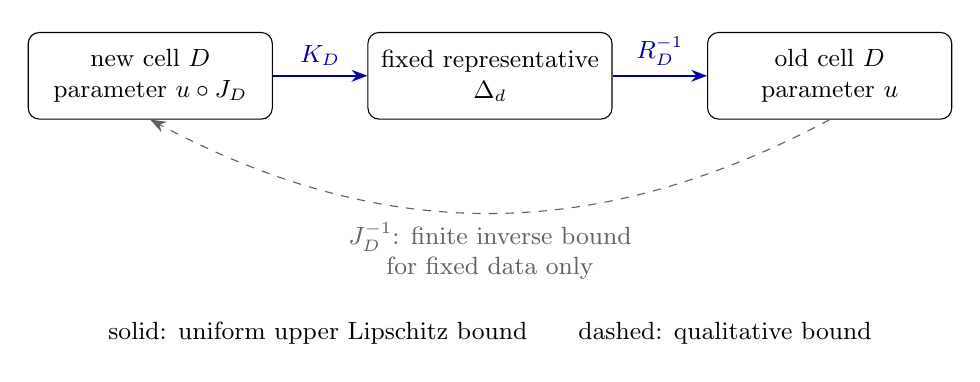
\begin{tikzpicture}[
  box/.style={draw,rounded corners,align=center,minimum width=3.1cm,
              minimum height=1.1cm,font=\small},
  bounded/.style={-{Stealth[length=2mm]},thick,blue!65!black},
  qualitative/.style={-{Stealth[length=2mm]},dashed,gray!75!black},
  every edge quotes/.style={font=\small}]
\node[box] (new) {new cell $D$\\parameter $u\circ J_D$};
\node[box,right=1.2cm of new] (rep) {fixed representative\\$\Delta_d$};
\node[box,right=1.2cm of rep] (old) {old cell $D$\\parameter $u$};
\draw[bounded] (new) -- node[above,font=\small] {$K_D$} (rep);
\draw[bounded] (rep) -- node[above,font=\small] {$R_D^{-1}$} (old);
\draw[qualitative] (old.south) to[bend left=28]
 node[below,font=\small,align=center] {$J_D^{-1}$: finite inverse bound\\for fixed data only} (new.south);
\node[below=2.45cm of rep,font=\small,align=center]
 {solid: uniform upper Lipschitz bound\qquad dashed: qualitative bound};
\end{tikzpicture}
\end{document}
